\subsection{\emph{ROS 2 Middleware Implementations}}
\label{subsec:rmw}

\emph{ROS 2 middleware implementations} (RMW) merupakan implementasi dari sistem komunikasi \emph{middleware} yang ada pada ROS 2,
  menggantikan TCPROS/UDPROS yang ada pada ROS yang sebelumnya \citep{url:rmwdesign}.
Pada ROS 2, \emph{middleware} yang digunakan berbasis pada sistem yang dimiliki oleh DDS,
  dimana DDS sendiri memiliki berbagai macam implementasi seperti RTI Connext DDS \citep{url:rmwdesign} eProsima Fast DDS \citep{url:fastdds},
  Eclipse Cyclone DDS \citep{url:cyclonedds},
  dan sebagainya.

Seperti yang terlihat pada gambar \ref{fig:diagramsistemros2},
  sistem komunikasi yang ada pada ROS 2 terdiri atas \emph{user application} di bagian paling atas,
  kemudian \emph{ROS 2 client library} (RCL) dengan implementasi bahasanya masing-masing,
  dan terakhir RMW yang terhubung dengan berbagai macam implementasi DDS.
Di sini, peran RMW adalah sebagai penghubung antara RCL dengan implementasi DDS yang digunakan.
Sehingga komunikasi pada tingkat \emph{middleware} seperti \emph{publish/subscribe} dengan QoS, \emph{discovery},
  dan \emph{graph event} dapat dilakukan terlepas dari implementasi yang digunakan.

Saat ini ROS 2 sudah mendukung beberapa implementasi DDS yang bisa digunakan sebagai RMW dari sistem yang digunakan.
  Implementasi tersebut dibentuk sebagai \emph{ROS 2 package} seperti pada \emph{package} \lstinline{rmw_connextdds} yang digunakan untuk menjalankan implementasi DDS dari RTI Connext DDS,
  \emph{package} \lstinline{rmw_fastrtps} yang digunakan untuk menjalankan implementasi DDS dari eProsima Fast DDS,
  dan lain sebagainya.

\begin{sidewaysfigure}[!htb]
  \centering
  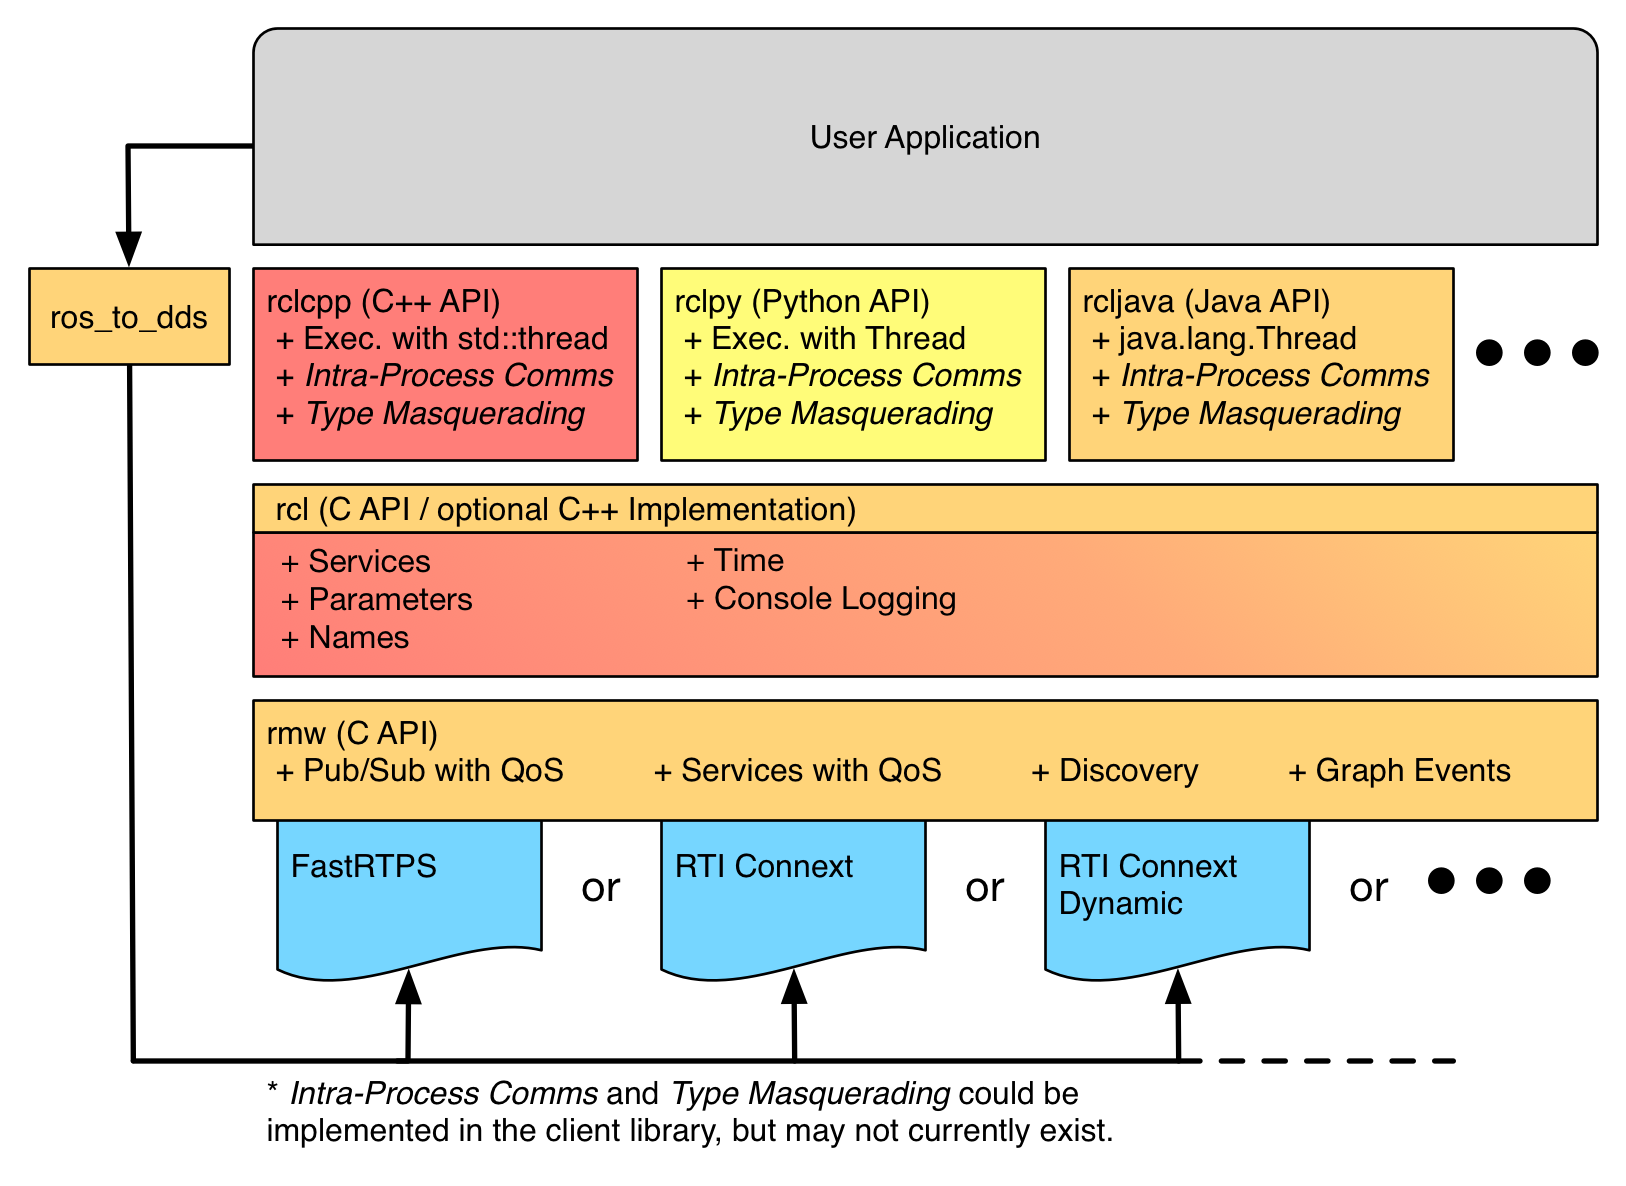
\includegraphics[width=0.8\textwidth,keepaspectratio]{gambar/diagram-sistem-ros2.png}
  \caption{Diagram sistem yang ada pada ROS 2 \citep{url:ros2interfacesconcept}.}
  \label{fig:diagramsistemros2}
\end{sidewaysfigure}
